\documentclass[]{standalone}
%\documentclass[dvisvgm]{minimal}

\usepackage[]{tikz}
\usepackage{sfmath}
\usepackage{pgfplots}
\pgfplotsset{compat=1.16}

\renewcommand{\familydefault}{\sfdefault}

\usetikzlibrary{positioning, fit}

\ifstandalone
\providecommand{\figurepath}{../figures}
\fi

\begin{document}
\begin{tikzpicture}[>=stealth, mybox/.style={thick, rounded corners, inner sep=4}]
  \node [mybox, draw=black] (parameter) {Parameter};
  \node [mybox, draw=black, right=0.5cm of parameter] (model) {Model};
  \node [mybox, draw=black, right=0.8cm of model] (data) {Data};
  \node [below=0.2cm of data] (plus) {\textbf{+}};
  \node [mybox, draw=black, below=0.2cm of plus] (noise) {Noise};

  \node [mybox, draw=black, dashed, fit={(data) (noise)}] (noisy_data) {};

  \path [->, thick] (parameter.east) edge (model.west)
    (model.east) edge (data.west)
    ([yshift=-0.8cm] noisy_data.west) edge[out=180, in=-90, red] node[below]
    {Inference} (parameter.south);

  % \node [very thick, draw=black, fit={(parameter) (model) (noisy_data)}] () {};

  \node [above=0.1cm of parameter.north west]
    {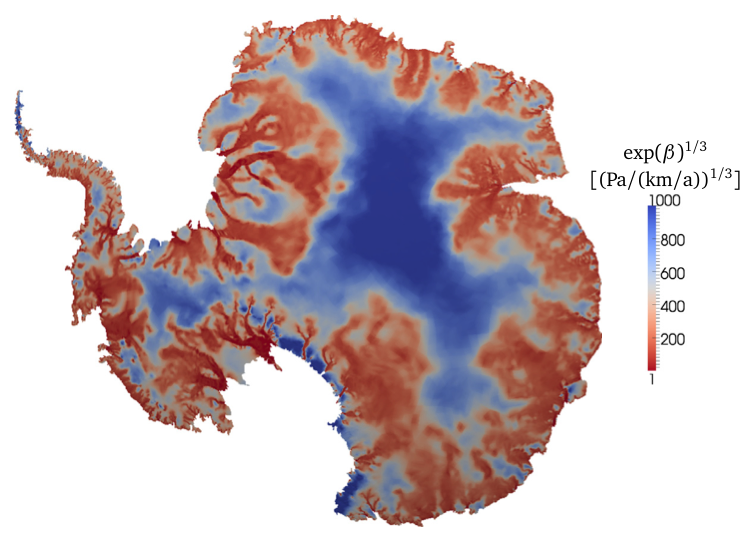
\includegraphics[scale=.2]{\figurepath/Antarctic_basal_sliding_parameter.png}};
  \node [above=0.5cm of noisy_data.north east]
    {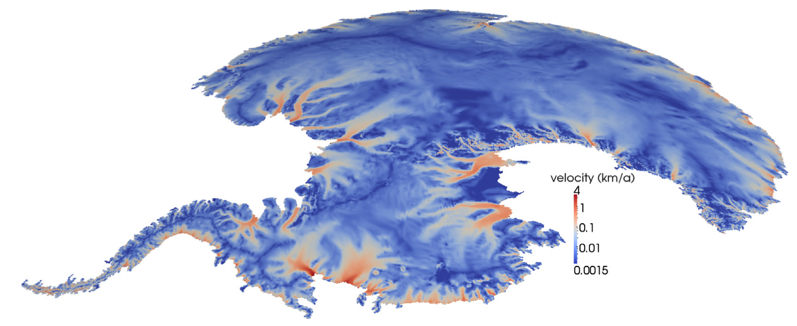
\includegraphics[scale=.2]{\figurepath/Antarctic_surface_velocity.png}};

\end{tikzpicture}
\end{document}
